\section{Isis\-Dlm.cpp File Reference}
\label{IsisDlm_8cpp}\index{IsisDlm.cpp@{IsisDlm.cpp}}
{\tt \#include $<$cstdio$>$}\par
{\tt \#include $<$iostream$>$}\par
{\tt \#include $<$fstream$>$}\par
{\tt \#include $<$string$>$}\par
{\tt \#include $<$list$>$}\par
{\tt \#include $<$vector$>$}\par
{\tt \#include \char`\"{}Idl.h\char`\"{}}\par
{\tt \#include \char`\"{}Idl\-Dlm.h\char`\"{}}\par
{\tt \#include \char`\"{}Idl\-Rtn\-Def.h\char`\"{}}\par
{\tt \#include \char`\"{}Idl\-Utilities.h\char`\"{}}\par
{\tt \#include \char`\"{}File\-Repository.h\char`\"{}}\par
{\tt \#include \char`\"{}Isis\-Dlm.h\char`\"{}}\par
{\tt \#include \char`\"{}Isis\-Dlm\-Routines.h\char`\"{}}\par


Include dependency graph for Isis\-Dlm.cpp:\begin{figure}[H]
\begin{center}
\leavevmode
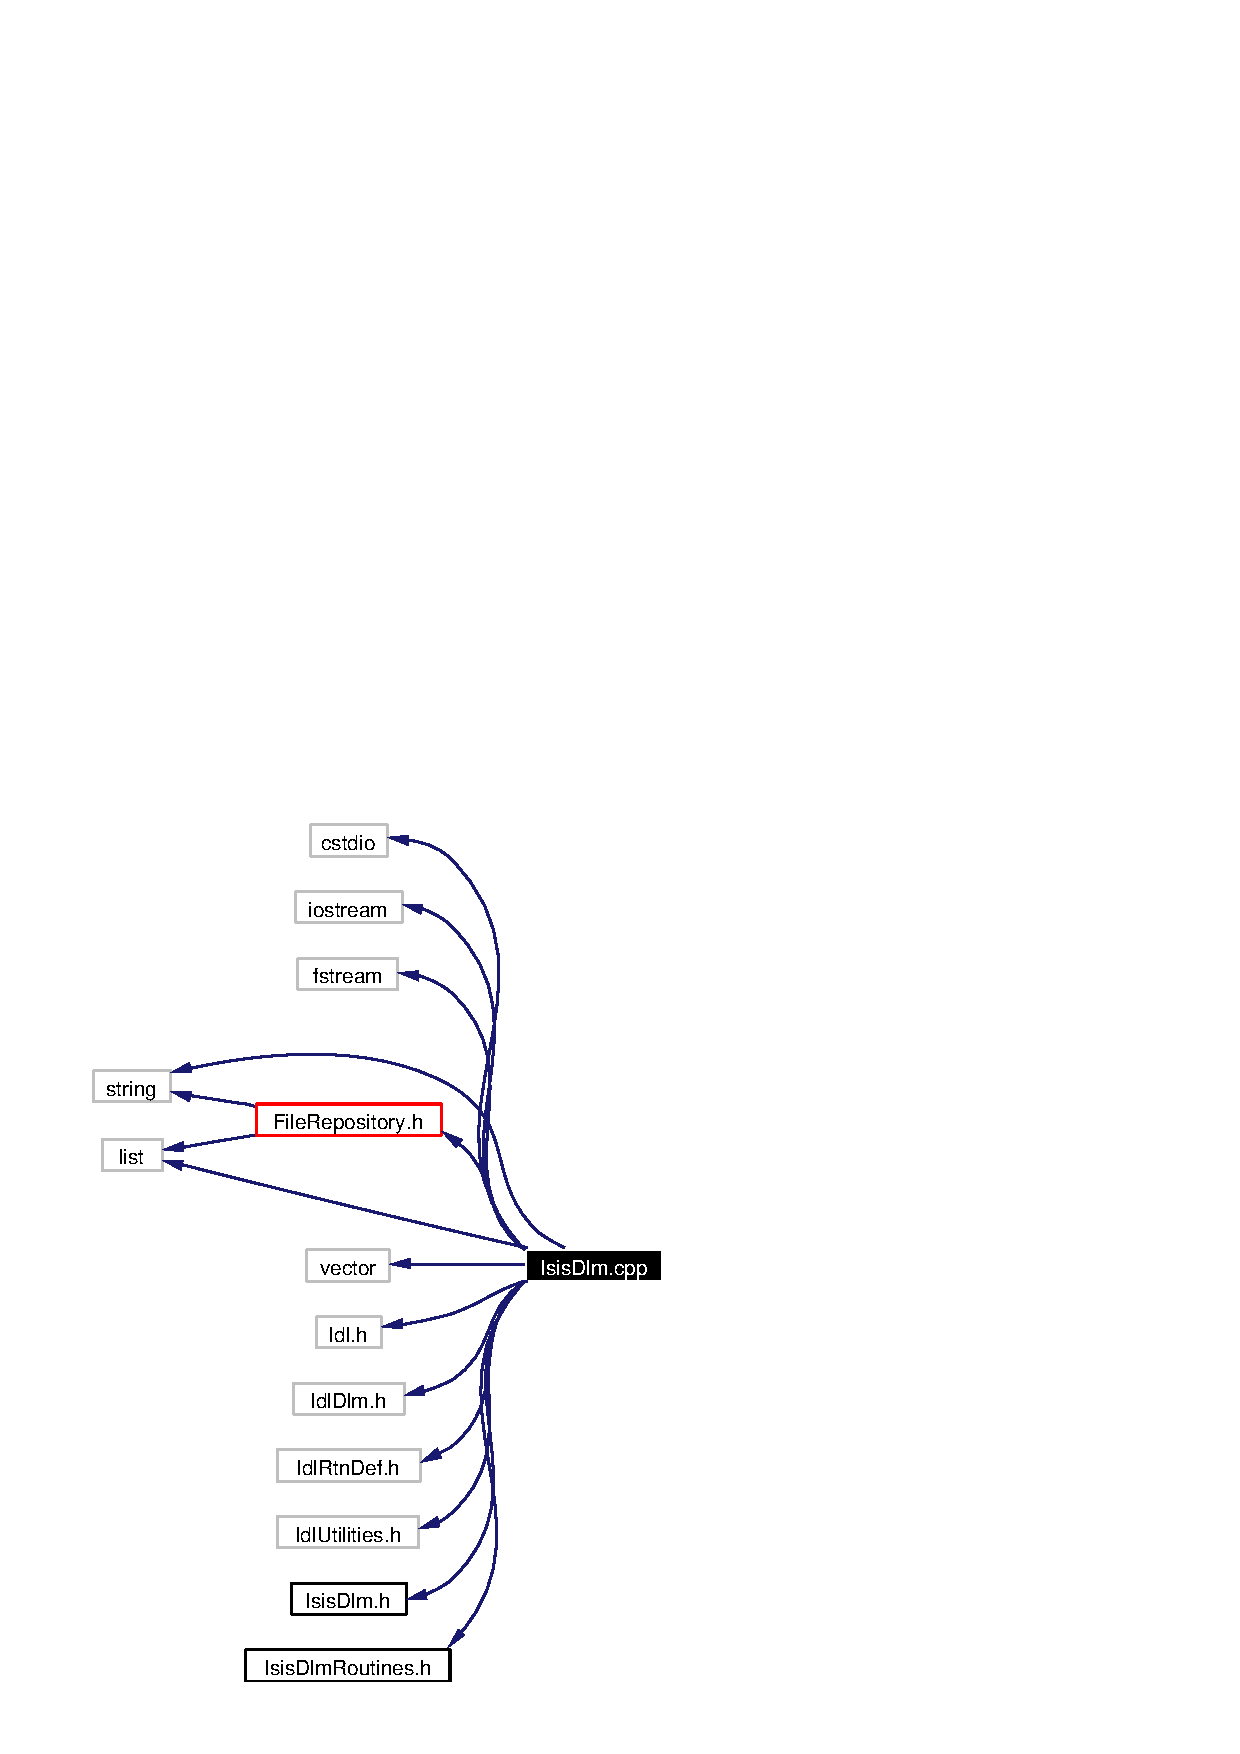
\includegraphics[width=163pt]{IsisDlm_8cpp__incl}
\end{center}
\end{figure}
\subsection*{Defines}
\begin{CompactItemize}
\item 
\#define {\bf MAKE\_\-INIT\_\-LIST}
\end{CompactItemize}
\subsection*{Functions}
\begin{CompactItemize}
\item 
int {\bf Isis\-Terminate} (void)
\item 
int {\bf Idl\-Init} (Idl\-Dlm \&idl)
\end{CompactItemize}


\subsection{Define Documentation}
\index{IsisDlm.cpp@{Isis\-Dlm.cpp}!MAKE_INIT_LIST@{MAKE\_\-INIT\_\-LIST}}
\index{MAKE_INIT_LIST@{MAKE\_\-INIT\_\-LIST}!IsisDlm.cpp@{Isis\-Dlm.cpp}}
\subsubsection{\setlength{\rightskip}{0pt plus 5cm}\#define MAKE\_\-INIT\_\-LIST}\label{IsisDlm_8cpp_a0}




\subsection{Function Documentation}
\index{IsisDlm.cpp@{Isis\-Dlm.cpp}!IdlInit@{IdlInit}}
\index{IdlInit@{IdlInit}!IsisDlm.cpp@{Isis\-Dlm.cpp}}
\subsubsection{\setlength{\rightskip}{0pt plus 5cm}int Idl\-Init (Idl\-Dlm \& {\em idl})}\label{IsisDlm_8cpp_a2}


{\bf IDL} DLM initialization routine This routine is called precisely when the first routine in the ISIS DLM is called from the {\bf IDL} calling environment. It performs the following operations:\begin{itemize}
\item Names the DLM - in this case its {\em Isis\/}\item Registers all the functions defined in the Isis\-Dlm.dlm file\item Registers the exit hander, Isis\-Terminate in this case\end{itemize}
One unfortunate consequence of the {\bf IDL} DLM is that you must be very careful should the routines defined in the DLM description file {\em Isis\-Dlm.dlm\/}. The Idl\-Dlm toolkit will disable all routines in this DLM should the initialization fail.

\begin{Desc}
\item[Parameters:]
\begin{description}
\item[{\em idl}]The Idl DLM interface system \end{description}
\end{Desc}
\begin{Desc}
\item[Returns:]0 if all registered OK, else then number of routines that failed \end{Desc}


Here is the call graph for this function:\begin{figure}[H]
\begin{center}
\leavevmode
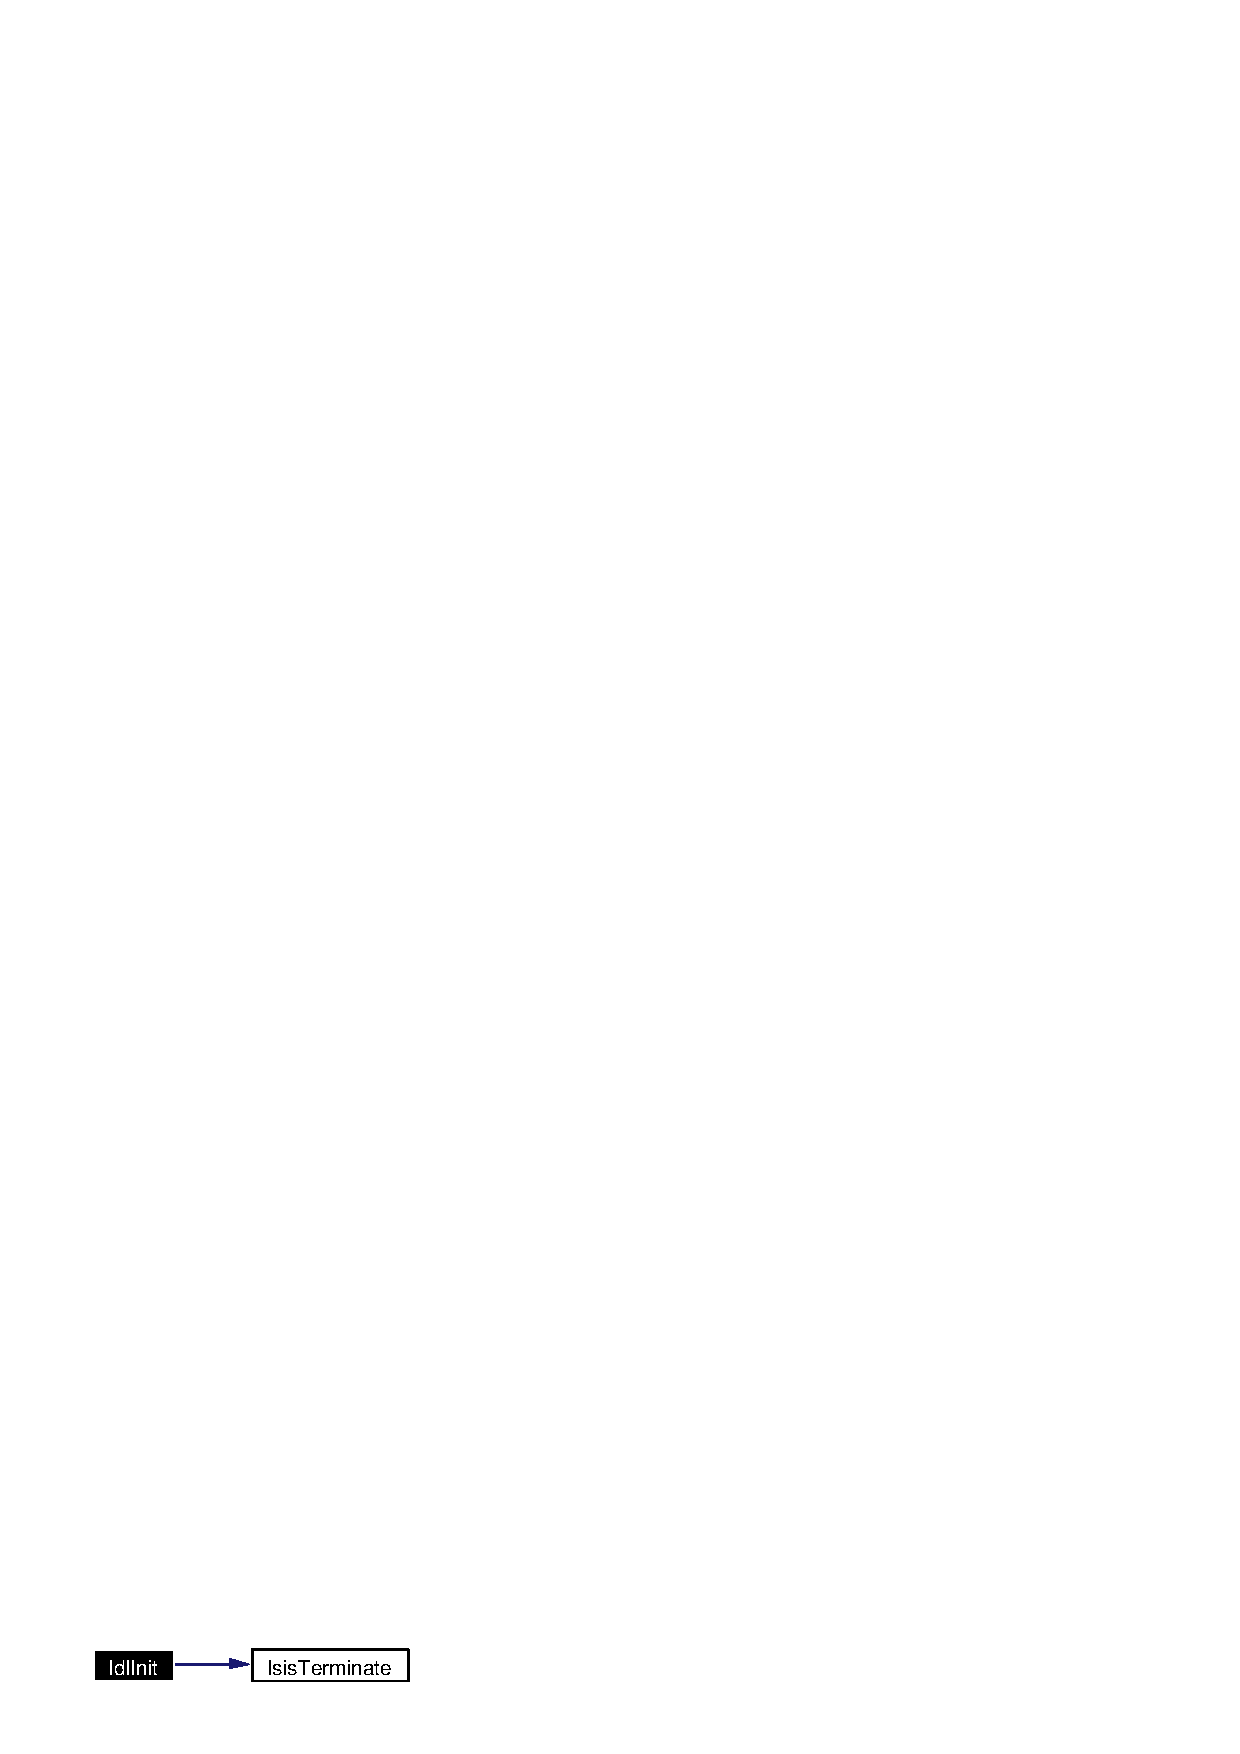
\includegraphics[width=102pt]{IsisDlm_8cpp_a2_cgraph}
\end{center}
\end{figure}
\index{IsisDlm.cpp@{Isis\-Dlm.cpp}!IsisTerminate@{IsisTerminate}}
\index{IsisTerminate@{IsisTerminate}!IsisDlm.cpp@{Isis\-Dlm.cpp}}
\subsubsection{\setlength{\rightskip}{0pt plus 5cm}int Isis\-Terminate (void)}\label{IsisDlm_8cpp_a1}


Exit routine for Isis\-Dlm internals Isis\-Terminate will be registered as an exit handler with the Idl\-Dlm toolkit. This routine is called once and only once precisely when {\bf IDL} is exiting. This is your last chance to do any clean up that is left prior to application termination. 